\subsection{Profil računovođe}

Računovođi se nakon uspešne prijave otvara profil. Prikaz profila računovođe je na slici \ref{fig:profilR}. 
Profil sadrži osnovne informacije o računovođi. Sa leve strane računovođa može da otvori stranice sa izveštajima, kao što su: pregled plata zaposlenih, pregled cena usluga, pregled uplata. 

\begin{figure}[H]
  \begin{center}
      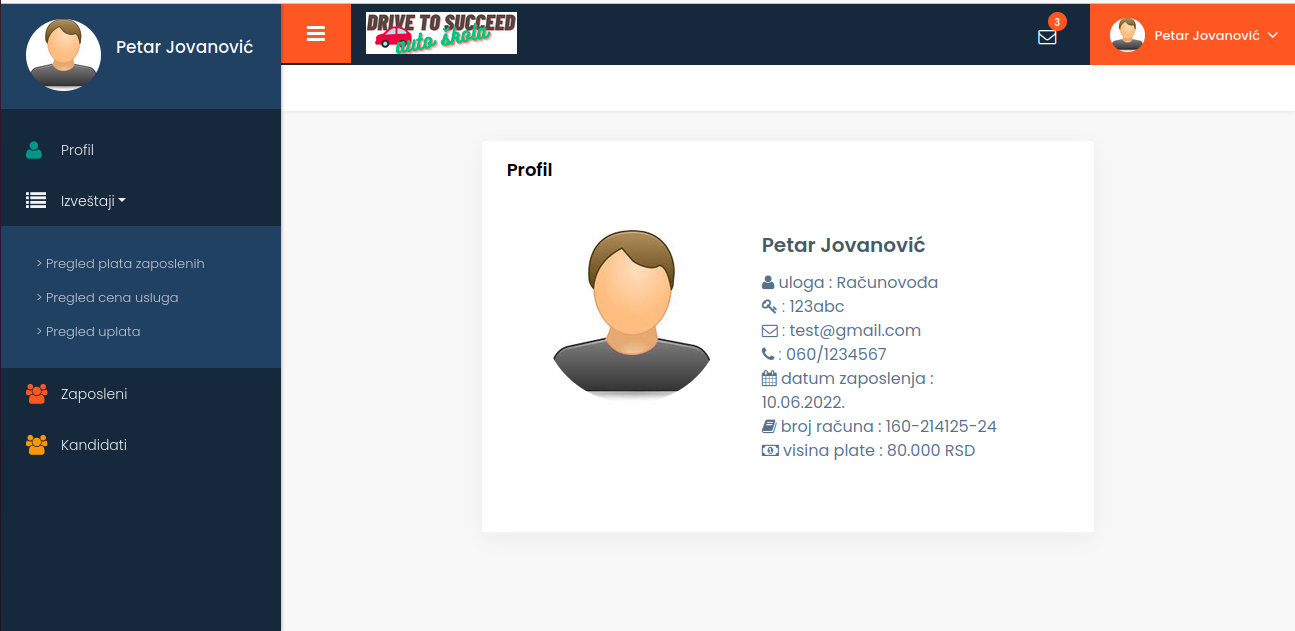
\includegraphics[width=140mm, height=60mm]{UI/UI_profil_racunovodja.png}
  \end{center}
  \caption {Profil računovođe}
  \label{fig:profilR}

\end{figure}

\subsection{Pregled uplata}

Stranica za prikaz uplata sadrži listu svih uplata. Date su osnovne informacije o uplatama u tabeli: Šifra uplate, uplatilac, iznos, datum uplate i svrha uplate.
  Računovođa ima opciju da izmeni uplatu i da obriše uplatu. Ako izabere opciju za brisanje uplate prikazuje se stranica, čiji je izgled dat na slici \ref{fig:ui_brisanje}. Računovođa ima i opciju za pretraživanje uplate. Izgled stranice za pregled uplata je prikazan na slici 
\ref{fig:ui_uplate}.

\begin{figure}[H]
  \begin{center}
      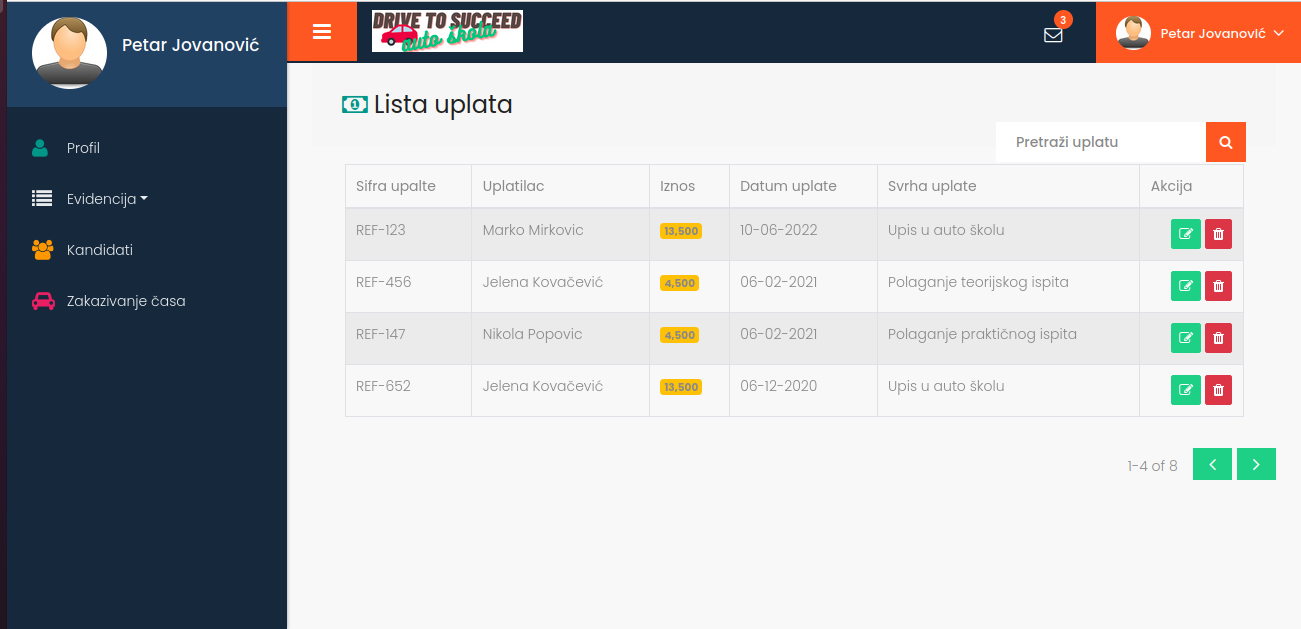
\includegraphics[width=140mm, height=60mm]{UI/UI_lista_uplata.png}
  \end{center}
  \caption {Lista uplata kandidata}
  \label{fig:ui_uplate}

\end{figure}



\begin{figure}[H]
  \begin{center}
      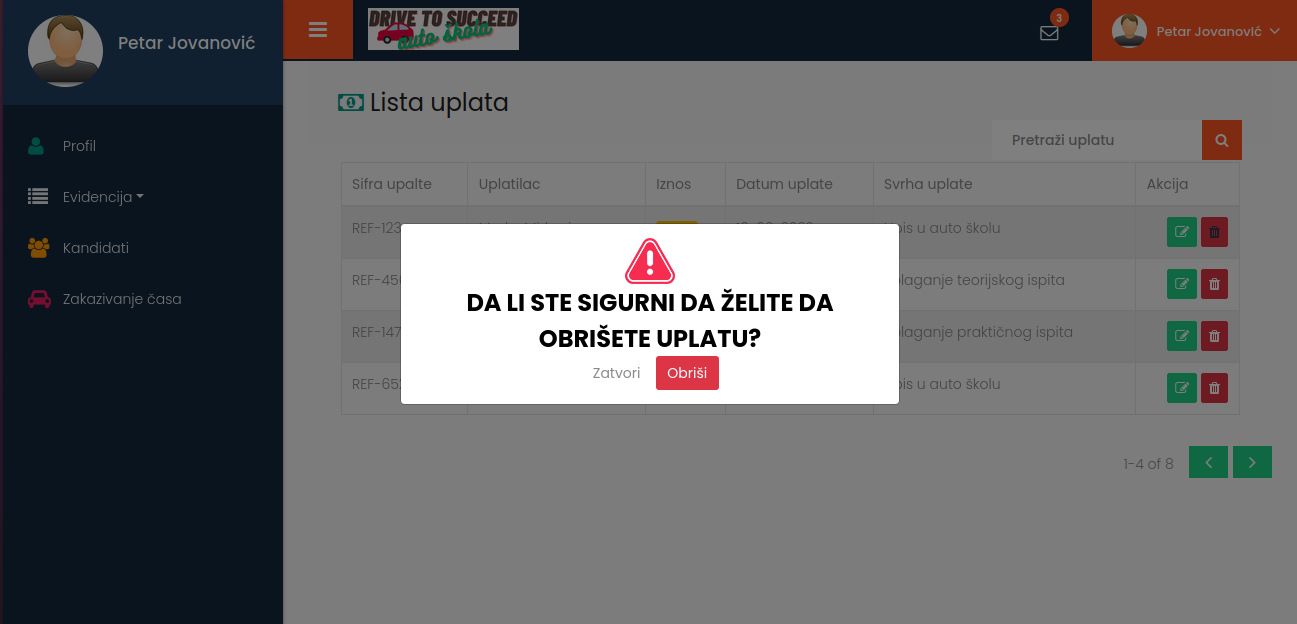
\includegraphics[width=140mm, height=60mm]{UI/UI_brisanje_uplate.png}
  \end{center}
  \caption {Brisanje uplate}
  \label{fig:ui_brisanje}

\end{figure}

